\section{Aggregation, Bag, Collection}
\label{sec:Aggregation,}
%%%%%%%%%%%%%%%%%%%%%%%%%%%%%%%%%%%%%%%%%%%%%%%%%%%%%%%%
\begin{figure}[h!]
\begin{center}
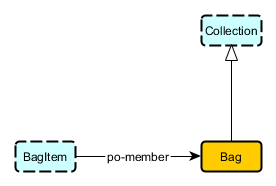
\includegraphics[width=.8\textwidth]{figures/aggregation}
\end{center}
\caption{Schema Diagram for the Aggregation, Bag, Collection Pattern. The visual notation is explained in Chapter \ref{chap:prelims}.}
\label{fig:Aggregation,}
\end{figure}
\subsection{Summary}
\label{sum:Aggregation,}
%%%%%%%%%%%%%%%%%%%%%%%%%%%%
The pattern for an Aggregation, Bag, or Collection is relatively simple. The Bag is a type of unordered collection. This pattern was included in this library for demonstrating a more approachable interface for the partonymy pattern, with respect to membership. For example, we may use this pattern to represent a committee. In this case, the committee member is the\textsf{BagItem}, the committee is the \textsf{Bag}, and the \textsf{itemOf} property is a sub-property to the \textsf{po-member} property found in the Partonymy/Meronymy pattern (Section \ref{sec:Partonymy}). This pattern was adapted from the Bag ontology design pattern and be found at \url{http://ontologydesignpatterns.org/wiki/Submissions:Bag}. Some language is borrowed from the description.

%%%%%%%%%%%%%%%%%%%%%%%%%%%%%%%%%%%%%%%%%%%%%%%%%%%%%%%%
\subsection{Axiomatization}
\label{axs:Aggregation,}
%%%%%%%%%%%%%%%%%%%%%%%%%%%%
\begin{align}
% General Axioms
\textsf{Bag} &\sqsubseteq \textsf{Collection} \\
\textsf{itemOf} &\sqsubseteq \textsf{po-member} \\
% Domain and Range Restrictions
\exists\textsf{itemOf.BagItem} &\sqsubseteq \textsf{Bag} \\
\textsf{Bag} &\sqsubseteq \forall\textsf{itemOf.BagItem} \\
% Inverse Aliases (if any) 
\end{align}

%%%%%%%%%%%%%%%%%%%%%%%%%%%%%%%%%%%%%%%%%%%%%%%%%%%%%%%%
\subsection{Explanations}
\label{exp:Aggregation,}
%%%%%%%%%%%%%%%%%%%%%%%%%%%%
\begin{enumerate}
\item Subclass: a \textsf{Bag} is a \textsf{Collection}
\item Subproperty: \textsf{itemOf} is a subproperty to \textsf{po-member} from the Partonymy Pattern (Section \ref{sec:Partonymy}).
\item Scoped Domain: the scoped domain of \textsf{itemOf}, scoped by \textsf{BagItem}, is \textsf{Bag}.
\item Scoped Range: the scoped range of \textsf{itemOf}, scoped by \textsf{Bag}, is \textsf{BagItem}.
\end{enumerate}

%%%%%%%%%%%%%%%%%%%%%%%%%%%%%%%%%%%%%%%%%%%%%%%%%%%%%%%%
\subsection{Competency Questions}
\label{cqs:Aggregation,}
%%%%%%%%%%%%%%%%%%%%%%%%%%%%
\begin{enumerate}[CQ1.]
\item What bag is this item an element of?
\item What resource does this item refer to?
\item What are the items contained in this bag?
\end{enumerate}

\newpage
%%%%%%%%%%%%%%%%%%%%%%%%%%%%%%%%%%%%%%%%%%%%%%%%%%%%%%%%
% End Section
%%%%%%%%%%%%%%%%%%%%%%%%%%%%%%%%%%%%%%%%%%%%%%%%%%%%%%%%
%%%%%%%%%%%%%%%%%%%%%%%%%%%%%%%%%%%%%%%%%%%%%%%%%%%%%%%%